\section{Results}
% \subsection{Demonstration of improved oracle tracking and orbital stability}
\subsection{Oracle Tracking Performance and Orbital Stability}
% \begin{itemize}
%     \item Show results for learning periodic motions on 2D "toy-like" datasets (e.g., star, rectangle, circle, etc.).
%     \item Demonstrate how our approach is a) more accurate at tracking the oracle than the prior work that used a Hausdorff loss~\citep{zhi2024teaching} and b) more stable than black-box machine learning models such as NeuralODEs or RNNs.
%     \item Include both plots of the learned velocity fields and a table that contains the quantitative evaluation results.
% \end{itemize}

% First, we compare the performance of \glspl{OSMP} with several baseline methods. These include traditional ML approaches for parameterizing motion policies, such as \glspl{RNN}, and \glspl{NODE}~\citep{chen2018neural}, as well as existing stable motion primitives for periodic movements like \gls{SPDT}~\citep{zhi2024teaching}. 
% In the case of \gls{RNN}, we consider a five-layer network that is trained to predict the velocity of the system based on the given demonstrations. Similarly, we define the \gls{NODE}~\cite{chen2018neural} as a five-layer \gls{MLP} with a hidden dimension of $128$ and Leaky ReLUs serving as the nonlinearities that predict the desired velocity of the system. During training, we integrate the system for $100$ steps using forward Euler and compute the loss of the trajectory positions against the demonstration.
% Furthermore, we benchmark against \gls{SPDT}, which notably employs a similar formulation as the proposed \gls{OSMP} but relies on the Hausdorff loss instead of our proposed limit cycle matching loss when training the motion primitive.
% As datasets, we consider a variety of motion behaviors that are based on oracles defined by simple, closed, two-dimensional geometric shapes, such as a star and a Dolphin shape. Furthermore, we evaluate the learning on the MIT CSAIL logo and the more intricate TU Delft flame logo.
First, we compare the performance of \glspl{OSMP} against several baseline methods. These include traditional \gls{ML} approaches for parameterizing motion policies, such as \glspl{RNN} and \glspl{NODE}~\citep{chen2018neural}, as well as existing \glspl{SMP} for periodic movements like \gls{SPDT}~\citep{zhi2024teaching}. For the \gls{RNN}, we employ a five-layer network with a hidden dimension of $128$ trained to predict the system’s velocity based on the provided demonstrations. Similarly, the \gls{NODE} is defined as a five-layer \gls{MLP} with a hidden dimension of $128$ and Leaky ReLUs serving as the nonlinearities to predict the desired system velocity. During training, we integrate the system for 100 steps using forward Euler and compute the loss based on the trajectory positions compared to the demonstration. Additionally, we benchmark against \gls{SPDT}, which notably uses a formulation similar to the proposed \gls{OSMP} but relies on the Hausdorff distance~\citep{hausdorff1914grundzuge} loss instead of our proposed limit cycle matching loss during training. As datasets, we consider a variety of motion behaviors based on oracles defined by simple, closed, two-dimensional geometric shapes, such as a star and a Dolphin shape, and further evaluate the learning on the MIT CSAIL logo as well as the more intricate TU Delft flame logo.

\begin{figure}[ht!]
    \centering
    \includegraphics[width=1.0\linewidth]{osmp/figures/benchmarking_results/benchmarking_results_v1_cropped_compressed.pdf}
    \caption{\textbf{Benchmarking the oracle tracking performance and orbital stability of \glspl{OSMP}.}
    In this figure, we display the qualitative benchmarking results when comparing the proposed \gls{OSMP} against baseline methods, such as \glspl{RNN}, \glspl{NODE}~\citep{chen2018neural}, or \gls{SPDT}~\citep{zhi2024teaching}. The various columns represent different geometric shape-based oracles on which the motion policies were trained, shown as white dotted lines on the plots. The color map and the streamlines denote the velocity of the learned motion policy when evaluated on a grid. We initialize the trained motion policies at 10 different randomly sampled initial conditions and roll out their trajectory, visualized using solid green lines, for a duration of one period.
    }
    \label{fig:osmp:benchmarking_results}
\end{figure}

% The results presented in Fig.~\ref{fig:osmp:benchmarking_results} show that the proposed \gls{OSMP} exhibits superior convergence and stability characteristics compared to motion policies without physical structure, such as \glspl{RNN} or \glspl{NODE}. Specifically, for the relatively simple case of the star shape, most trajectories still converge to the periodic demonstration, but we notice some spurious attractors in the center of the star shape. For more complex oracles such as the TU Delft flame or the Dolphin oracle, the \gls{RNN} and the \gls{NODE} based motion policies are not able to track the demonstration in a stable fashion.
% While \gls{SPDT}~\citep{zhi2024teaching} exhibits the same stability and convergence guarantees as \gls{OSMP}, we notice a much-improved precision of \glspl{OSMP} at shaping the limit cycle such that it accurately matches the given periodic oracle. While this can already be noticed for the star oracle, this is particularly apparent for the TU Delft flame and Dolphin oracles.
The results in Fig.~\ref{fig:osmp:benchmarking_results} demonstrate that the proposed \gls{OSMP} offers superior convergence and stability compared to motion policies lacking physical structure, such as \glspl{RNN} or \glspl{NODE}. In the relatively simple case of the star shape, most trajectories converge to the periodic demonstration, although some spurious attractors appear inside the limit cycle. For more complex oracles, like the TU Delft flame or Dolphin shapes, the \gls{RNN}- and \gls{NODE}-based motion policies fail to track the demonstration in a stable fashion. While \gls{SPDT}~\citep{zhi2024teaching} provides similar stability and convergence guarantees to \gls{OSMP}, we observe that \gls{OSMP} achieves much higher precision in shaping the limit cycle to accurately match the given periodic oracle—a difference that is evident even in the star oracle and especially pronounced for the TU Delft flame and Dolphin oracles.

\subsection{Stable Tracking of Oracles Across Robot Embodiments}
% \begin{itemize}
%     \item Demonstrate how our proposed method is able to generate stable and accurate trajectories on a large variety of real-world robots.
%     \item Show experimental results for trajectory tracking on UR5 (robotic manipulator), KUKA (cobot), Helix (continuum soft robot), and joint-space and task-space turtle (rigid-soft underwater robot).
%     \item Possibly include comparisons with traditional trajectory tracking controllers to demonstrate that our learned motion primitive does not exhibit worse tracking accuracy.
% \end{itemize}

While the previous section focused on evaluating and benchmarking the learning of the \gls{OSMP}, we now aim to demonstrate that the proposed \gls{OSMP} can effectively control robot motion in real-world scenarios. To achieve this, we apply the method to a diverse range of robot embodiments, including robot manipulators (UR5), \glspl{Cobot} (KUKA), soft robots (Helix Robot)~\citep{guan2023trimmed}, and prototypes of hybrid soft-rigid underwater robots (Crush turtle robot).

\begin{figure}[h!]
    \centering
    \includegraphics[width=1.0\linewidth]{osmp/figures/robot_embodiments_results/robot_embodiments_results_v1_cropped.pdf}
    \caption{\textbf{Stable tracking of oracles across robot embodiments in the real world.}
    This figure shows the trajectories of various robot embodiments controlled with \glspl{OSMP} based on data recorded during real-world experiments.
    The first row shows the behavior of a UR5 manipulator in task space where the \gls{OSMP} is trained on various geometric shape oracles, including an ellipse, a square, and a doge. The black dotted lines denote the oracle, the orange line is the actual trajectory of the UR5's end-effector, and the velocity field is based on the learned \gls{OSMP}.
    The second row considers the same trained \glspl{OSMP}, but this time evaluates their behavior on a Helix soft robot.
    The third row presents the behavior of traditional trajectory tracking controllers on the Helix soft robot for the same oracles.
    Finally, the fourth row contains measurements of the Crush turtle robot operated (in water) by \glspl{OSMP} trained on biological oracles, where the black dotted line denotes the oracle and the colored line the actual behavior of the right flipper arm. In the first and third, the forward swimming (biological)~\citep{van2022new} and reverse swimming oracles, respectively, are directly defined in joint space~\citep{van2023soft}. The second row shows a \gls{OSMP} applied to a biological forward swimming oracle defined in task space, which, in this case, corresponds to the tip position and twist angle (not visible here) of the right flipper arm.
    }
    \label{fig:osmp:robot_embodiments_results}
\end{figure}

Figure~\ref{fig:osmp:robot_embodiments_results} illustrates the effectiveness of OSMPs across all tested robot embodiments. 
% Here, the OSMP operates in task space and outputs desired task space velocities. Subsequently, we modify the robot's low-level controllers (task space) setpoint by incrementing the end effector position based on the desired velocity and the used time step.
Here, the OSMP operates in task space, outputting the desired task space velocities. Next, we update the robot’s low-level controller setpoint by incrementing the end effector’s position based on the desired velocity and the applied time step.
For the UR5 manipulator, we observe precise trajectory tracking. Although the Helix soft robot is also capable of tracking the trajectory, hysteresis effects and inaccuracies in its kinematic model—which lead to incorrect actuation inputs from the inverse kinematics—result in some oscillatory behavior and imprecision. It is important to note that this is not an inherent limitation of the \gls{OSMP} method but rather an issue that similarly affects traditional trajectory tracking methods, as it can be seen that the trajectory tracking controller, defined in \eqref{eq:osmp:trajectory_tracking_controller}, exhibits steady-state errors and in parts of the trajectory even instability.

In addition, we pursue learning swimming behavior for the Crush Turtle robot using biological oracles. Specifically, our objective is to have the \gls{OSMP} control the two front flipper arms—the primary tools for turtle swimming. We employ both a three-dimensional oracle defined in joint space~\citep{van2023soft} and a four-dimensional oracle defined in task space (comprising the flipper tip position and twist angle)~\citep{van2022new}, both derived from video recordings of green sea turtles (Chelonia mydas)~\citep{van2022new, van2023soft}. Subsequently, the commanded joint space velocities are tracked by the actuators.
These instances illustrate that \glspl{OSMP} can learn oracles with dimensions exceeding $n=2$. In real-world pool experiments, we observe that \glspl{OSMP} enable the Crush Turtle robot to accurately track the trajectory at moderate speeds. When the period of the periodic trajectory is shortened by increasing $\omega$, the motor’s acceleration and velocity constraints prevent perfect tracking, particularly during the faster segments of the oracle. Nonetheless, even if the motion diverges from the oracle, stability is maintained, and the system consistently returns to the oracle.

\begin{figure}
    \centering
    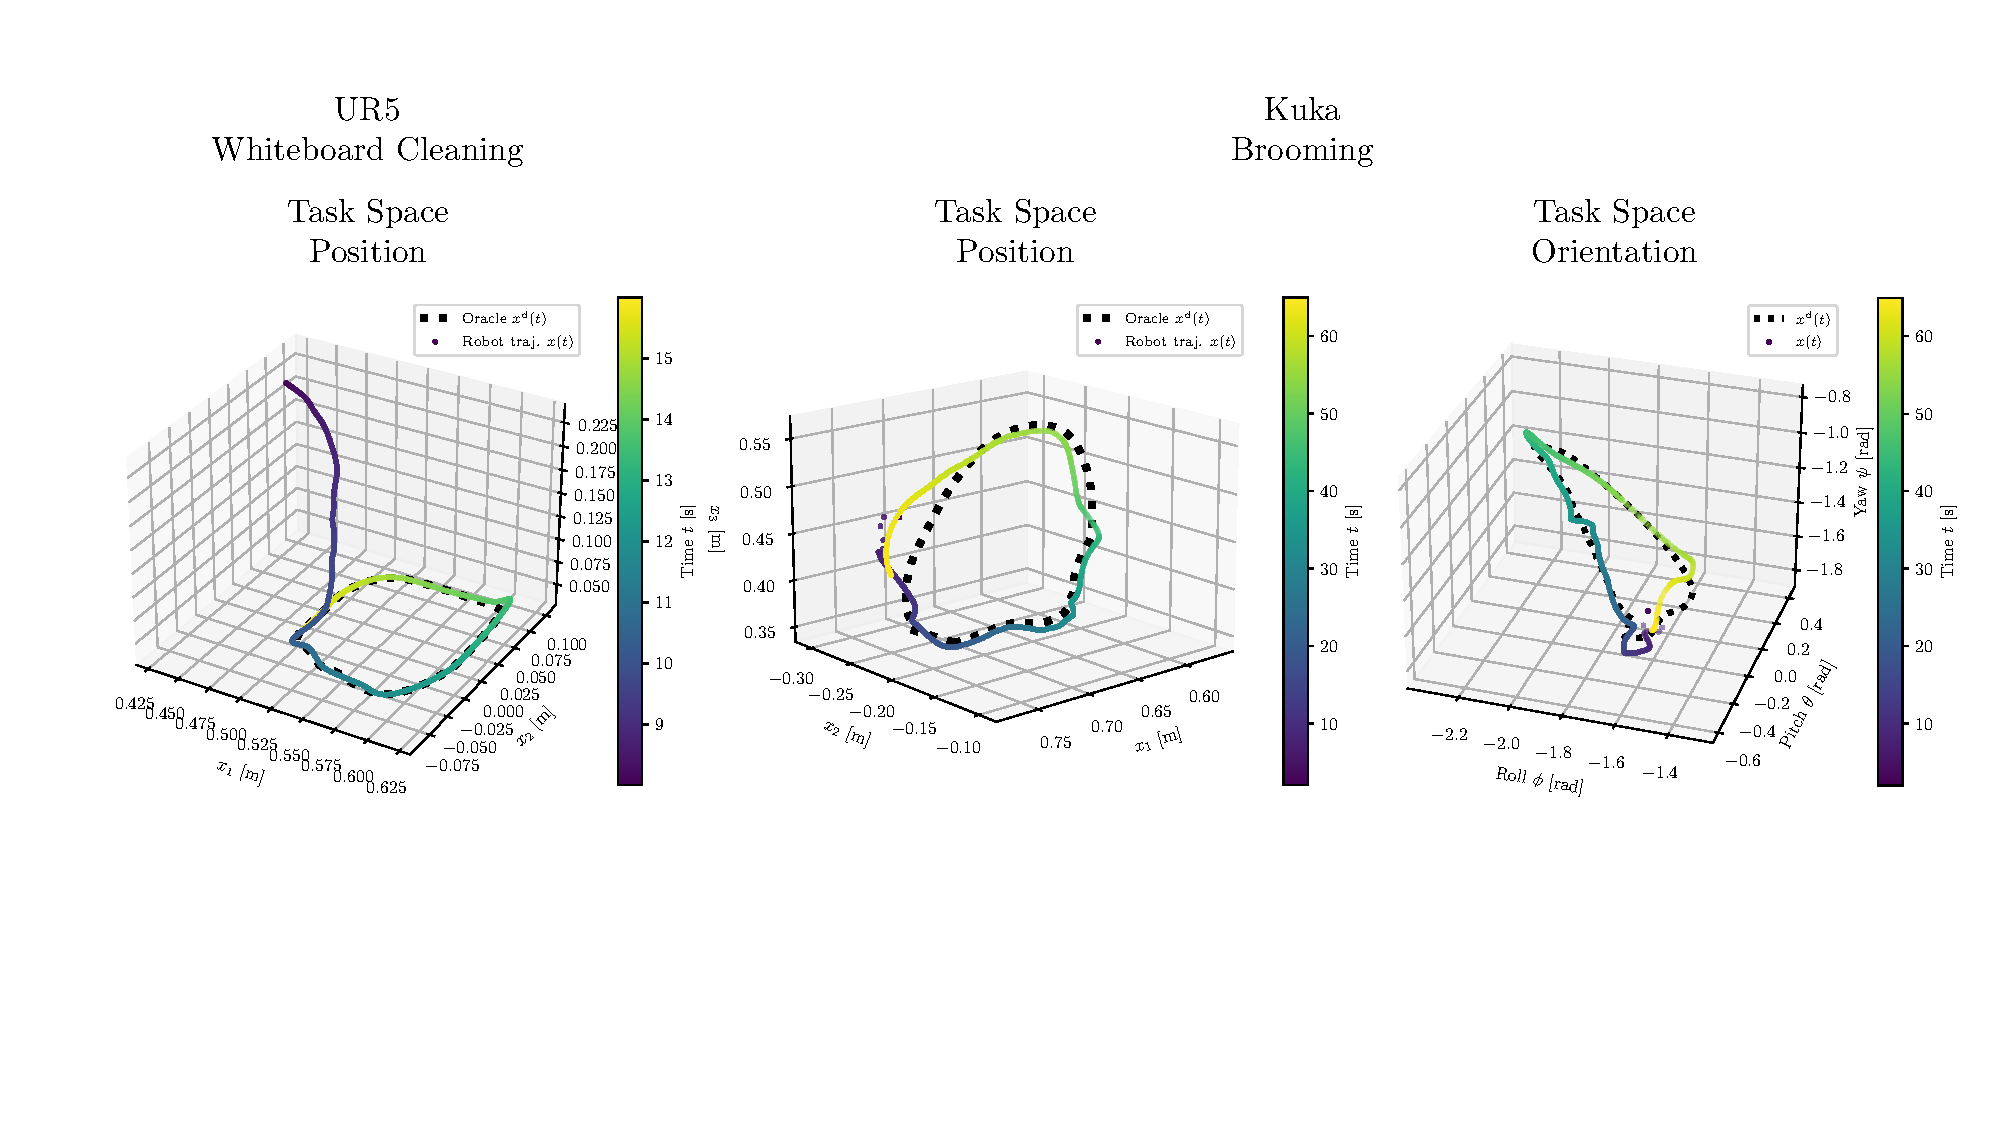
\includegraphics[width=1.0\linewidth]{osmp/figures/kinesthetic_teaching_results/kinesthetic_teaching_results_v1_cropped.pdf}
    \caption{\textbf{Real-world results for learning orbital motion primitives from kinesthetic demonstrations.}
    In the first column, we show the results for a whiteboard cleaning task executed with the UR5 manipulator, and in the second and third columns, we show the results for a booming task executed with the KUKA robot.
    In both cases, the demonstration was provided via kinesthetic teaching, and the \gls{OSMP} was trained on the resulting periodic oracle.
    For the UR5 manipulator, the \gls{OSMP} learns the motion of the end-effector position in three dimensions. For the KUKA manipulator, we learn both the motion of the end-effector position and orientation.
    The color signifies the time when executing the task using the trained \gls{OSMP}.
    }
    \label{fig:osmp:kinesthetic_teaching_results}
\end{figure}

\subsection{Learning Orbital Motion Primitives from Kinesthetic Demonstrations}
% \begin{itemize}
%     \item Demonstrate how our method is able to be applied to demonstrations that were created using kinesthetic teaching and that it is able to accomplish real-world tasks.
%     \item Show results for UR5 whiteboard cleaning and KUKA brooming tasks.
% \end{itemize}

In this section, we examine demonstrations captured through kinesthetic teaching, which tend to be more jerky and less smooth compared to the well-defined geometric oracles discussed earlier. Moreover, when demonstrating periodic motion, the oracle usually does not perfectly close, as a spatial offset remains between the starting and ending poses, which makes it more challenging to fit the limit cycle to the oracle accurately

In Fig.~\ref{fig:osmp:kinesthetic_teaching_results}, we present results for learning \glspl{OSMP} on cleaning tasks that were provided via kinesthetic teaching. Specifically, we consider a whiteboard erasure task on a UR5 manipulator and a brooming task on a KUKA cobot.
While in the case of the UR5, we only encode the spatial translation (i.e., positions) of the end-effector in the \gls{OSMP}, we also consider the motion of the end-effector orientation in the case of the KUKA task. 
In the case of the UR5 robot, we observe a fast convergence onto the limit cycle and, subsequently, good tracking of the oracle with only minor deviations at the point where we fused the start/end points of the periodic motions.
When deploying the \gls{OSMP} on the KUKA \gls{Cobot}, we notice a larger tracking error - likely due to the challenging oracle with $n=6$ \glspl{DOF} and the low feedback gains used in the low-level controller.


\begin{figure}[h]
    \centering
    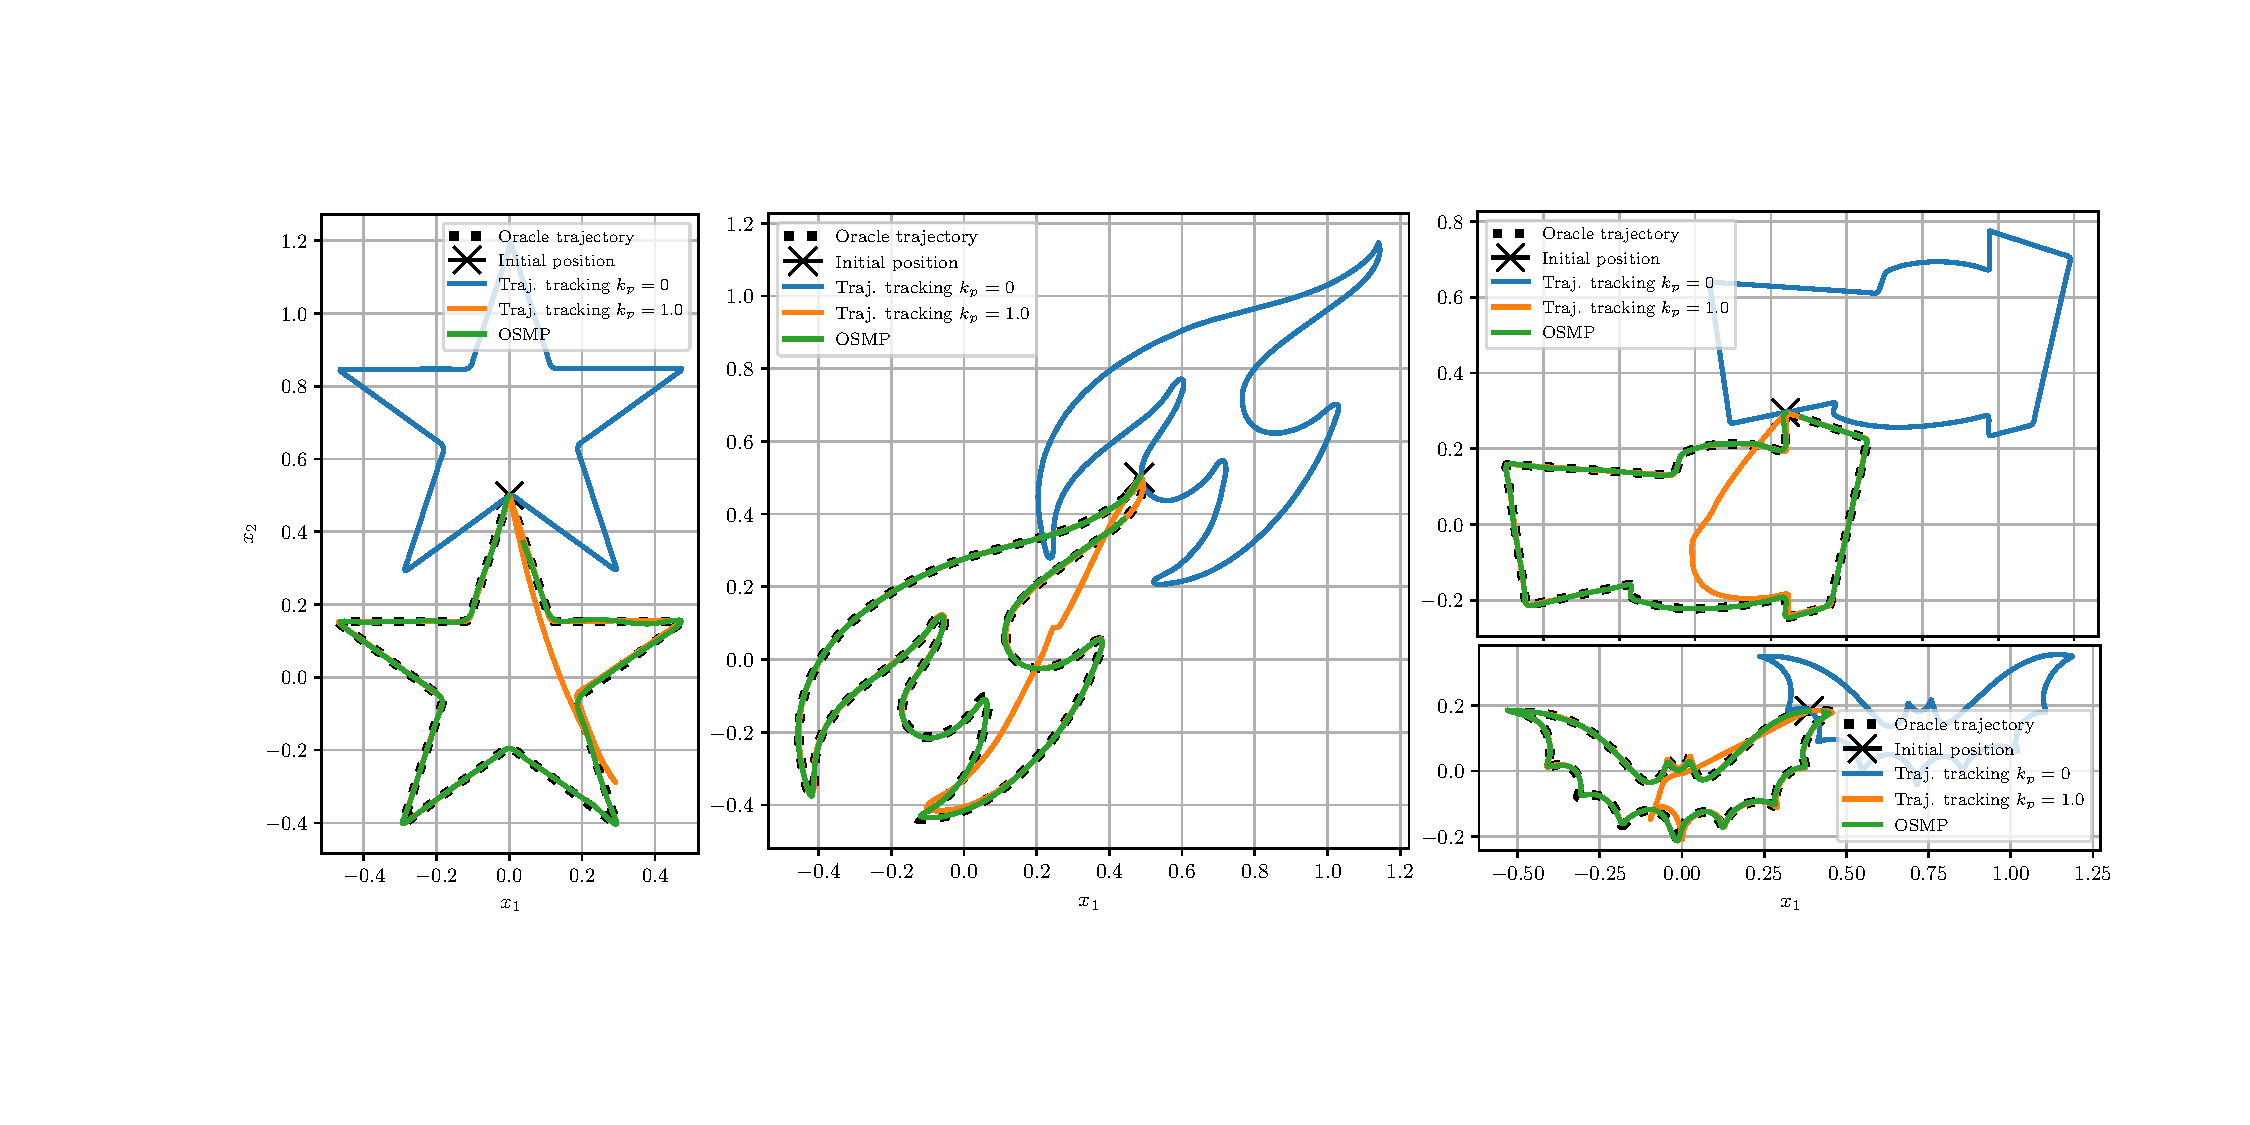
\includegraphics[width=1.0\linewidth]{osmp/figures/compliance_results/compliance_results_v1_cropped.pdf}
    \caption{\textbf{Analyzing the compliance and motion behavior.}
    Simulations with time perturbations where we compare the behavior of traditional, time-parametrized trajectory tracking controllers against the \glspl{OSMP}. Here, the dashed black lines denote the oracles/demonstrations, the solid blue lines the behavior of a pure feedforward trajectory tracking controller $\dot{x}(t) = \dot{x}^\mathrm{d}(t)$ operating on a time-parametrized reference $\dot{x}^\mathrm{d}(t)$, the orange line the behavior of an error-based feedback trajectory tracking controller $\dot{x}(t) = \dot{x}^\mathrm{d}(t) + k_\mathrm{p} \, (x^\mathrm{d}(t) - x(t))$ with $k_\mathrm{p} = 1$, and the green line the behavior of the learned \gls{OSMP}. Compared to nominal scenarios, we perturb the time reference - i.e., the time reference exhibits a $\pi$ offset in phase with respect to the initial position.
    }
    \label{fig:osmp:compliance_results}
\end{figure}

\subsection{The Learned Policies Exhibit Compliant and Natural Motion Behavior}
% \begin{itemize}
%     \item The goal of this subsection is to show how a policy parametrized by a dynamic system is much more compliant and exhibits more natural and predictable motions than a traditional time-parametrized trajectory tracking controller.
%     \item Show a simulated 2D toy case where we perturb the time reference. Then, we compare the trajectories of a) a time-parametrized pure feedforward controller, b) a time-parametrized feedforward+feedback controller, and c) our orbital motion primitive. The feedforward controller would diverge upon time perturbation, the feedforward+feedback controller would be able to track the trajectory but exhibit unnatural motions, and the motion primitives are not affected by a perturbation in the time reference.
%     \item Show the results of the real-world experiments where the dynamical motion primitive exhibited a much more compliant behavior upon physical interaction of the robot than the time-parametrized trajectory tracking controller.
% \end{itemize}

We aim for robots in human-centric environments to demonstrate robust, compliant, and predictable behavior. Specifically, \emph{robustness} means that if a robot deviates from its intended path—perhaps due to a disturbance—it will always converge back to the desired motion. \emph{Compliance} indicates that robots should exert only minimal forces when coming into contact with humans, and \emph{predictability} ensures that their motions are sufficiently consistent for humans to anticipate their behavior and respond appropriately.

In this section, we compare the reaction upon disturbances and perturbations of \glspl{OSMP} against traditional trajectory tracking controllers that rely on a time-parametrized trajectory.
Such error-based feedback controllers are usually given in the form
\begin{equation}\label{eq:osmp:trajectory_tracking_controller}
    \dot{x}(t) = \dot{x}^\mathrm{d}(t) + K_\mathrm{p} \, (x^\mathrm{d}(t) - x(t)),
\end{equation}
where $K_\mathrm{p} \in \mathbb{R}^{n \times n}$ is a proportional feedback gain that operates on the error between the current position $x(t)$ and the desired position $x^\mathrm{d}(t)$. In practice, we choose a scalar $k_\mathrm{p} \in \mathbb{R}_+$ such that $K_\mathrm{p} = k_\mathrm{p} \, \mathbb{I}_{n}$. We stress here the reliance on a time-parametrized trajectory provided in the form $(x^\mathrm{d}(t),\dot{x}^\mathrm{d}(t)) \: \forall \: t \in [t_0, t_\mathrm{f}]$. 
We evaluate in simulation three motion controllers: a pure feedforward trajectory tracking controller, which we gather by setting $k_\mathrm{p} = 0$, and an error-based feedback controller with $k_\mathrm{p} > 0$, and the learned \gls{OSMP}.
In this setting, we are particularly interested in analyzing the behavior of the motion controllers upon encountering an external disturbance that perturbs the state of the system with respect to the time reference. For this, we shift the time reference when initializing the system by half a period (i.e., a phase shift of $\pi$~rad).

The results in Fig.~\ref{fig:osmp:compliance_results} show that the pure feedforward trajectory tracking controller entirely drifts off the desired trajectory. When adding an error-based feedback term, the traditional trajectory tracking controller is able to recover and rejoin the demonstrated trajectory after a bit. However, while doing so, the feedback term generates a very aggressive correction action, which could cause incompliant behavior and would not seem natural to humans. Instead, the \gls{OSMP}, which is solely conditioned on the system state and not time, is not affected by the perturbation of the time reference and perfectly tracks the demonstration while exhibiting compliant and natural behavior.


\subsection{Achieving Phase Synchronization Across Multiple Motion Primitives}
% \begin{itemize}
%     \item Motivate why phase synchronization is important and for which applications it can be useful.
%     \item Showcase a 2D toy example where we are synchronizing three or more learned motion primitives.
%     \item Show the real-world results from the turtle pool tests where i) the turtle doesn't swim when the flippers are not synchronized, ii) how we achieve the flipper synchronization and how that makes the turtle swim.
% \end{itemize}

In many practical applications, such as locomotion, synchronizing multiple motion policies is critical. In this section, we illustrate how our approach can synchronize multiple learned \glspl{OSMP} by evaluating the polar phase of each and then aligning them via an error-based feedback controller~\citep{dorfler2014synchronization}. Crucially, we only adjust the velocity magnitude without altering the system’s spatial motion, thereby preserving the imitation and convergence properties of each learned motion policy.

\begin{figure}[h]
    \centering
    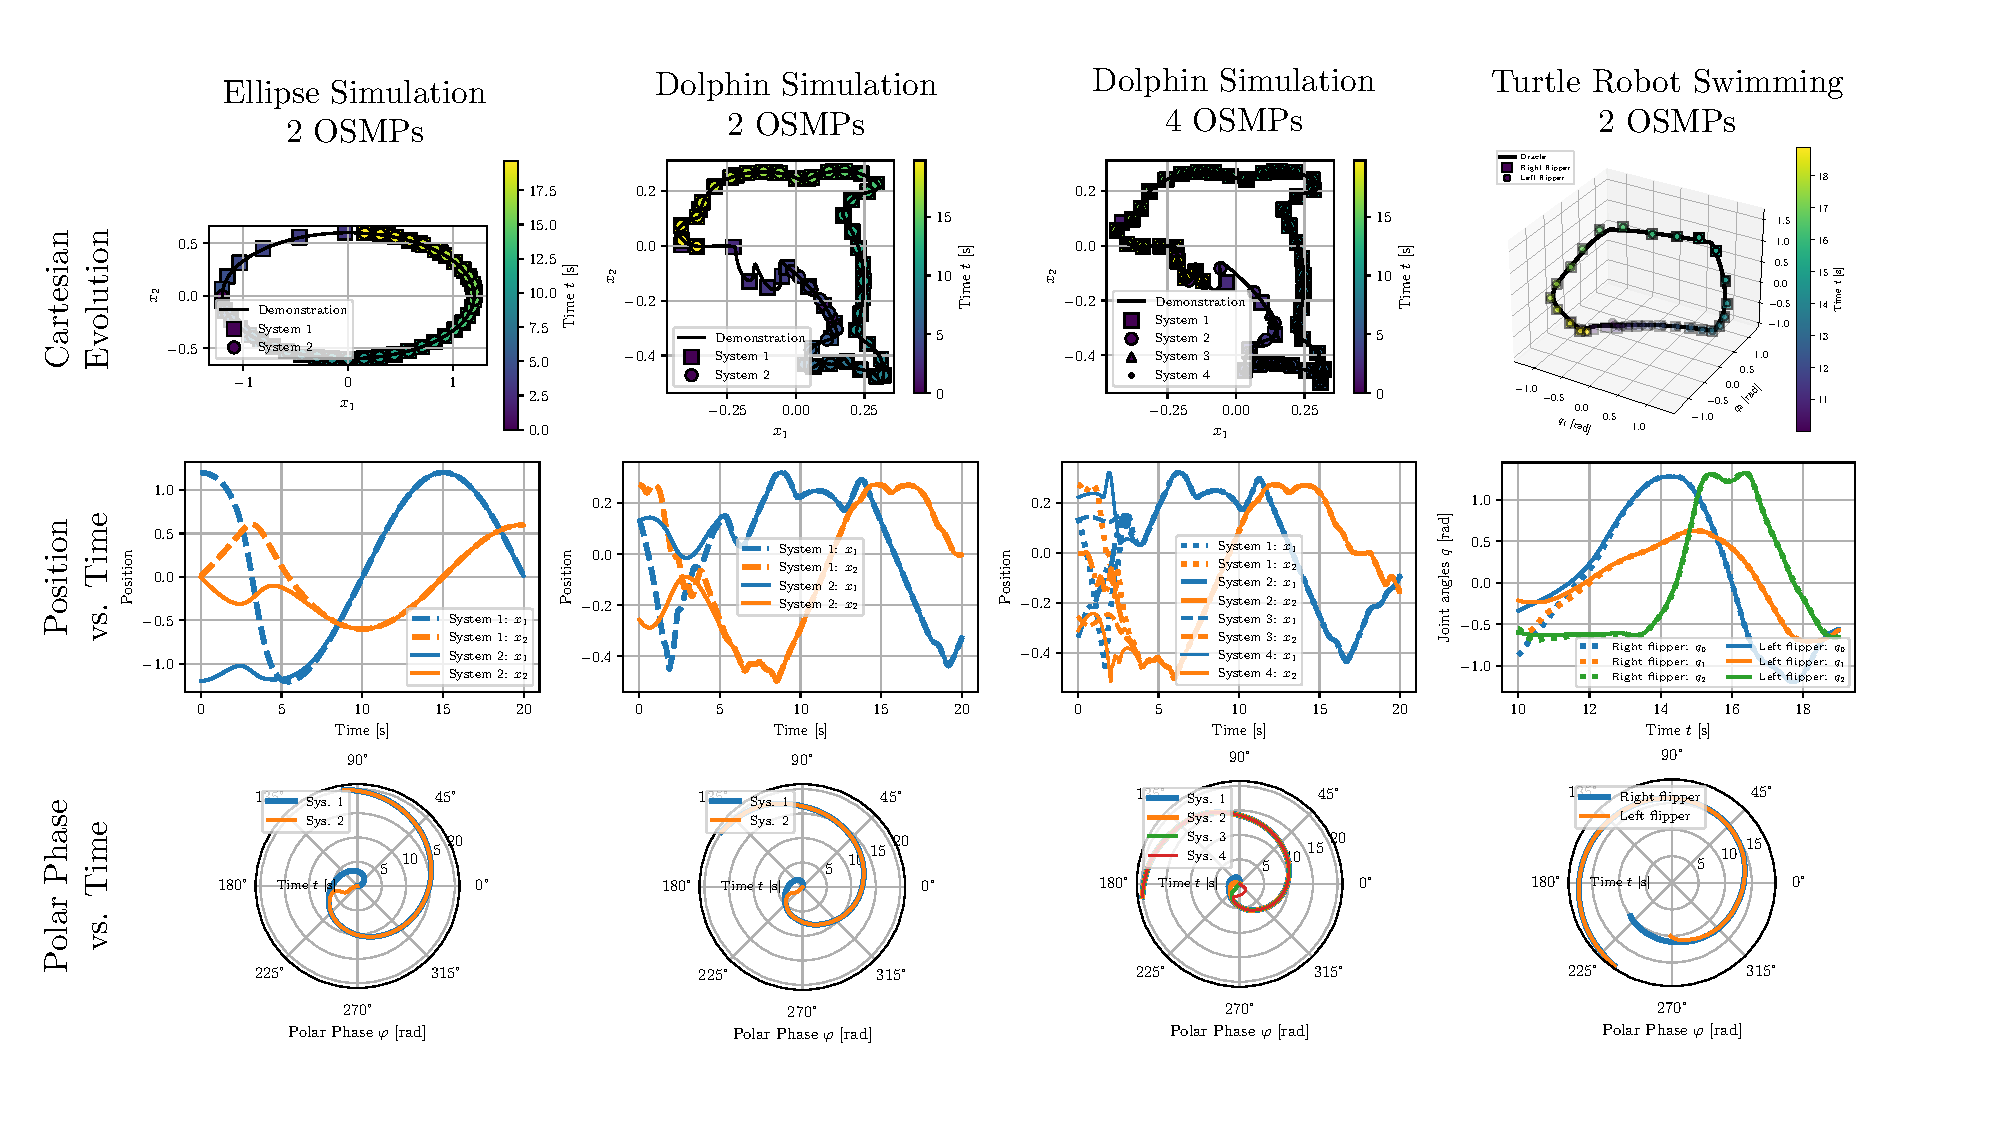
\includegraphics[width=1.0\linewidth]{osmp/figures/phase_sync_results/phase_sync_results_v1_cropped.pdf}
    \caption{\textbf{Phase synchronization of \glspl{OSMP}.}
    Results for the phase synchronization of multiple \gls{OSMP} systems. The first row shows the Cartesian-space evolution of each \gls{OSMP}, where the color of the markers communicates the time information. The second row shows the position vs. time, and the last row shows the polar phase $\varphi$ of the systems over time. 
    The first three columns show simulation results for \glspl{OSMP} trained on ellipse and Dolphin demonstrations, respectively. In all rows, we synchronize the motion of two systems/\glspl{OSMP}, except for the third row, where we synchronize four systems.
    }
    \label{fig:osmp:phase_sync_results}
\end{figure}

In Fig.~\ref{fig:osmp:phase_sync_results}, we show simulation and experimental results for synchronizing two and four \glspl{OSMP}. The outcomes illustrate how the controller identifies the most efficient strategy to align the \glspl{OSMP}, achieving rapid polar phase synchronization. A proportional gain determines the aggressiveness of the synchronization process. The simulation results confirm that the phase synchronization approach is effective not only for two systems but also for four or more.

Regarding experimental findings, we examined the swimming performance of the Crush turtle robot. Tests in a swimming pool revealed that the robot can swim effectively only when both front flippers—the primary means of locomotion in water~\citep{van2022new, van2023soft}—are fully synchronized. In practice, even aside from external disturbances and inherent differences between the flippers, desynchronization occurs already during initialization when the flipper arms start in slightly different configurations with varying polar phases. Our results show that using our method, the two flipper arms synchronize in less than a quarter of a period, thereby enabling the turtle robot to swim effectively.

\subsection{Smooth Interpolation Between Motion Behaviors via Encoder Conditioning}
% \begin{itemize}
%     \item Motivate how encoder conditioning enables the incorporation of multiple oracles in the same motion primitive.
%     \item Motivate why we would (ideally) want to achieve smooth interpolation between oracles.
%     \item Showcase 2D toy examples for the interpolation between two or more oracles. We also show that this works in the real world on the UR5 robot.
%     \item Demonstrate how we can learn both forward and reverse turtle swimming with the same motion primitive using encoder conditioning and how we can smoothly interpolate between the two motions.
% \end{itemize}

As we move toward generalist motion policies~\citep{o2024open, black2024pi0, gemini2025robotics}, the motion policy must integrate not just a single behavior but a range of diverse behaviors conditioned on the task, the robot’s state, and its perception of the environment. In particular, we aim to leverage in the future semantic encodings from sources like \glspl{VLM} as motion conditioning. However, this aspect has not been sufficiently explored within the realm of dynamic motion primitives. Moreover, there may be many scenarios where interpolating between two or more motion behaviors from the training set is beneficial, which is not supported by the current methods~\citep{rana2020euclideanizing, perez2023stable, perez2024puma, sochopoulos2024learning, zhi2024teaching}.
%
One example involves different surface cleaning motions, where the specific cleaning action is selected based on the surface material. In this case, the robot should be able to transition smoothly between cleaning motions when moving from one surface to another. Another example is locomotion: if oracles are available for walking on flat terrain and for stepping over steep stairs, then for obstacles or moderately steep, stair-like terrain, it may be beneficial to interpolate between these two oracles, while we would want to preserve the naturalness of the motion.

\begin{figure}[h]
    \centering
    \includegraphics[width=1.0\linewidth]{osmp/figures/conditioning_results/conditioning_results_v1_cropped.pdf}
    \caption{
    \textbf{Smooth interpolation between distinct motion behaviors via encoder conditioning.}
    Results demonstrating the conditioning of the encoder on multiple learned motion behaviors, including smooth interpolation between behaviors.
    The first row shows the behavior of an OSMP that was trained jointly on a horizontal ellipse ($z=0$) and a vertical ellipse ($z=1$).
    The second row shows the behavior of an OSMP that was trained jointly on a horizontal ellipse ($z=0$) and a square ($z=1$).
    The third row shows the behavior of an OSMP that was trained jointly on a square ($z=0$) and the MIT CSAIL logo ($z=1$).
    The first four columns present the simulated behavior for a constant conditioning $z$ between $z=0$ and $z=1$, where the black dashed line denotes the two oracles used for training and the green line the simulated trajectory that is a function of the velocity field for the given conditioning $z$.
    The fifth column contains a simulation where the conditioning is slowly increased, where the color indicates the conditioning $z$.
    Similarly, the sixth column includes real-world results obtained with a UR5 manipulator where the conditioning is slowly increased from $z=0$ at $t=0$ to $z=1$ at $t=140$~s. Here, the color indicates the time.
    }
    \label{fig:osmp:conditioning_results}
\end{figure}

In this work, we introduce task conditioning for the bijective encoder using a conditioning variable $z \in \mathbb{R}$. This variable enables us to select the desired motion behavior online by providing the appropriate $z$ value. Moreover, we train the \gls{OSMP} so that the learned motion policy smoothly interpolates between two or more motion behavior conditionings (e.g., $z=0$ and $z=1$). As shown in Fig.~\ref{fig:osmp:conditioning_results}, our simulations and real-world experiments with a UR5 manipulator demonstrate that (a) the same \gls{OSMP} can accurately learn multiple motion behaviors and (b) smooth interpolation between these behaviors is achievable by adjusting the conditioning. Importantly, switching between motion behaviors does not require an elaborate sequence; once a new $z$ is set, the \gls{OSMP}’s convergence guarantees ensure that the system quickly adapts to the new behavior.